\subsection{Circuito de Alimentación}

La única parte de la plataforma de la figura \ref{diag_detallado} que hace falta implementar entonces, es el circuito de alimentación, que se encarga de proveer las tensiones y corrientes necesarias para el funcionamiento de todos los circuitos auxiliares de la plataforma. Al estar la plataforma dividida en circuitos de potencia y circuitos de señal o digitales, ambos aislados galvánicamente entre sí, va a ser necesario implementar fuentes de alimentación separadas y aisladas para cada una de estas partes.\\

Por este motivo, se presenta la tabla \ref{tabla:resumen_alimentacion} que resume los requerimientos de alimentación de cada dispositivo de la plataforma, separando entre dispositivos de la parte de potencia y digital y por tensión de alimentación.\\

\setlength{\tabcolsep}{8pt}
\renewcommand{\arraystretch}{1.5}
\begin{table}[h]
\begin{center}
    \begin{tabular}{llrrr}
        {\SemiBold Tipo} & {\SemiBold Dispositivo} & {\SemiBold Tensión} [\unit{\volt}] & {\SemiBold Corriente} [\unit{\milli\ampere}] & {\SemiBold Total} [\unit{\milli\ampere}]\\
        \hline
        \multirow{4}{*}{Potencia} & 2ED21834-S06J (x2) & \num{10}-\num{20} & 2200 & 2200\\
        \cline{2-5}
         & ACPL-P480 (x4) & \num{5} & \num{12} & \multirow{3}{*}{43.5} \\
         & LM5056A & \num{5} & \num{7.5} & \\
         & ISO7242C (Lado 1) & \num{5} & \num{24} & \\
        \hline
        \multirow{4}{*}{Digital} & TMCS1100A4 & \num{5} & \num{6} & \multirow{3}{*}{331} \\
         & TMS320F28335 & \num{5} & \num{300} & \\
         & FT232BL & \num{5} & \num{25} & \\
         \cline{2-5}
         & ISO7242C (Lado 2) & \num{3.3} & \num{24} & 24
    \end{tabular}
    \caption{Resumen de requerimientos de alimentación de todos los dispositivos de la plataforma, separado por tipo y tensión de alimentación.}
    \label{tabla:resumen_alimentacion}
\end{center}
\end{table}

Para este proyecto, se va a conectar a la plataforma un circuito de alimentación externo no regulado, con nivel de tensión variable entre \SI[]{12}[]{\volt} y \SI[]{18}[]{\volt} aproximadamente, que vamos a llamar $V_{DDA}$. Dado que esta fuente es considerablemente ruidosa y los circuitos de señal son más sensibles al ruido (manejan niveles de tensión mucho menores), la fuente no regulada se conecta del lado de potencia de la plataforma, referenciado a la tierra del lado primario del convertidor, $GND_1$.\\

\subsubsection{Alimentación de Potencia}

Como se ve en la sección superior de la tabla \ref{tabla:resumen_alimentacion}, en los circuitos de potencia se necesitan únicamente dos niveles de tensión de alimentación para cuatro dispositivos distintos:\\

\begin{itemize}
    \item {\SemiBold Circuito de 10-20 V:} Alimentación de ambos drivers para MOSFET (2ED21834-S06J), que consumen \SI[]{2.2}[]{\ampere} entre los dos, por cortos períodos de tiempo. 
    \item {\SemiBold Circuito de 5 V:} Alimentación de los cuatro optoacopladores (ACPL-P480) que requieren \SI[]{12}[]{\milli\ampere} en total, del sensor de tensión/corriente (LM5056) que requiere \SI[]{7.5}[]{\milli\ampere}, y del lado de potencia del aislador para I\textsuperscript{2}C (ISO7242C) que requiere \SI[]{24}[]{\milli\ampere} de corriente. \SI[]{43.5}[]{\ampere} de consumo total en el circuito.\\
\end{itemize}

\paragraph{Circuito de 10-20 V}

Según su hoja de datos, el driver 2ED21834-S06J requiere una tensión de entre \SI[]{10}[]{\volt} y \SI[]{20}[]{\volt} en su pin de alimentación VCC, con corrientes transitorias de alrededor de \SI[]{1.1}[]{\ampere} por cada dirver para nuestra aplicación. Por esta razón, la {\Medium alimentación para este dispositivo viene directamente de la fuente externa no regulada}, con el agregado de un capacitor de bypass de \SI[]{4.7}[]{\micro\farad} en derivación para filtrar la corriente ruidosa que entrega la fuente externa.\\

\paragraph{Circuito de 5 V}

El resto de los dispositivos del circuito de potencia requieren algún tipo de tensión regulada (es decir que tiene una muy baja variación en el nivel de tensión que entrega). Por una cuestión de simplicidad de diseño, es preferible alimentar a todo con el mismo nivel de tensión, obviando la necesidad de circuitos adicionales. Entonces, observando los niveles de tensión de alimentación permitidos para estos tres dispositivos, se eligió una tensión estándar de \SI[]{5}[]{\volt} que es compatible con todos los dispositivos.\\

Para lograr esta tensión regulada de \SI[]{5}[]{\volt} se debe tomar la tensión no regulada $V_{DDA}$ y bajar su nivel de tensión. Para esto se utiliza un {\Medium regulador lineal}, que toma una tensión de entrada y entrega a la salida una tensión (regulada) de menor valor. Es esencialmente un convertidor CC-CC lineal, que funciona bajo el principio de un divisor resistivo, utilizando un transistor como resistencia variable como se explicó en la sección 2 del capítulo \ref{analisis}. Los requerimientos que este regulador debe cumplir son los siguientes:\\

\begin{itemize}
    \item Tensión de salida de \SI[]{5}[]{\volt}.
    \item Regulación de tensión de salida menor a \SI[]{500}[]{\milli\volt}.
    \item Tensión de entrada máxima mayor a \SI[]{20}[]{\volt}.
    \item Corriente de salida mayor a \SI[]{90}[]{\milli\ampere}.
    \item Es deseable la utilización de encapsulados pequeños de montaje superficial.\\
\end{itemize}

Cumpliendo estas especificaciones, se eligió el regulador lineal modelo {\Medium LM7805} de Fairchild Semiconductor, de tres terminales y \SI[]{1}[]{\ampere} de corriente máxima de salida. Se presenta a continuación una tabla con sus especificaciones.\\

\setlength{\tabcolsep}{7pt}
\renewcommand{\arraystretch}{1.5}
\begin{table}[H]
\begin{center}
    \begin{tabular}{llrrrrr}
    {\SemiBold Fabricante} & {\SemiBold Modelo} & $\mathbf{V_{O}}$ [\unit{\volt}] & {\SemiBold Regulación} [\unit{\milli\volt}] & $\mathbf{V_I}$ [\unit{\volt}] & $\mathbf{V_{Drop}}$ [\unit{\volt}] & $\mathbf{I_O}$ [\unit{\ampere}]\\
    \hline
    \makecell[l]{Fairchild \\ Semiconductor} & LM7805 & \num{5} & \num{100} &  \num{35} & \num{2} & \num{1}
    \end{tabular}
    \caption{Especificaciones del regulador lineal LM7805 de \SI[]{5}[]{\volt} de Fairchild Semiconductor.\textsuperscript{\cite{LM7805}}}
    \label{tabla:LM7805}
\end{center}
\end{table}

Dónde $V_O$ es la tensión de salida (regulada) nominal, la regulación es la máxima variación de tensión de salida, $V_I$ es la máxima tensión de entrada, $V_{Drop}$ es la tensión de \textit{dropout}, es decir la mínima diferencia de tensión que puede haber entre entrada y salida, e $I_O$ es la máxima corriente de salida.\\

\begin{figure}[h]
    \centering
    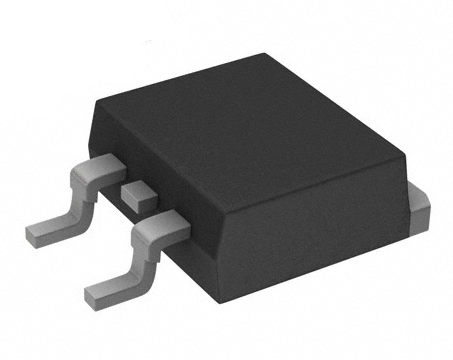
\includegraphics[scale=0.8]{Imagenes/D-PAK.png}
    \caption{Regulador lineal LM7805 de Fairchild Semiconductor, en su encapsulado de montaje superficial tipo D-PAK o TO-252.}
    \label{encapsulado_LM7805}
\end{figure}

Este regulador se consigue con el empaquetado SMD de tres pines de tipo D-PAK o TO-252 de la figura \ref{encapsulado_LM7805}. Incluye funcionalidades de seguridad como protección por sobre elevación térmica y cortocircuito, además de protección de operación en región segura del transistor de salida. Según recomendación del fabricante, se conectan dos capacitores por fuera del regulador: un capacitor de bypass de \SI[]{0.33}[]{\micro\farad} entre el pin de entrada y tierra, y otro capacitor de bypass de \SI[]{0.1}[]{\micro\farad} entre el pin de salida y tierra.\\

\subsubsection{Fuente Aislada}

Estando solucionada la alimentación de la parte de potencia de la plataforma, ahora se debe divisar una forma de obtener alimentación para la parte digital del circuito. Esta alimentación debe provenir de la alimentación externa no regulada $V_{DDA}$, pero al mismo tiempo estar aislada galvánicamente de la misma, utilizando la tierra $GND_D$ como referencia. Como ya se estableció, esto es necesario para evitar daños y prevenir la introducción de ruido no deseado a través de los pines de alimentación de los dispositivos.\\

Para este propoósito, vamos a utilizar un convertidor CC-CC regulado con aislación galvánica entre entrada y salida integrada en un único encapsulado. Esto reduce enormemente la complejidad de los circuitos de alimentación, pasando a ocupar mucho menos espacio y reduciendo su dependencia de tolerancias de circuitos de componentes discretos.\\

Particularmente, vamos a hacer uso de la fuente aislada {\Medium THB 3-1211} de Traco Power (una marca de Traco Electronic AG), un regulador lineal aislado de \SI[]{5}[]{\volt} y hasta \SI[]{600}[]{\milli\ampere} de salida. En la tabla \ref{tabla:TRACO} se presentan sus especificaciones más importantes.\\

\setlength{\tabcolsep}{7pt}
\renewcommand{\arraystretch}{1.5}
\begin{table}[H]
\begin{center}
    \begin{tabular}{llrrrrr}
    {\SemiBold Fabricante} & {\SemiBold Modelo} & $\mathbf{V_{O}}$ [\unit{\volt}] & {\SemiBold Regulación} & $\mathbf{V_I}$ [\unit{\volt}] & $\mathbf{V_{ISO}}$ [\unit{\volt}\textsubscript{RMS}] & $\mathbf{I_O}$ [\unit{\milli\ampere}]\\
    \hline
    Traco Power & THB 3-1211 & \num{5} & \num{0.5}\% &  \num{18} & \num{1000} & \num{600}
    \end{tabular}
    \caption{Especificaciones de la fuente CC-CC aislada THB 3-1211 de Traco Power.\textsuperscript{\cite{TRACO}}}
    \label{tabla:TRACO}
\end{center}
\end{table}

Dónde $V_O$ es la tensión de salida (regulada) nominal, la regulación es la máxima variación de tensión de salida, $V_I$ es la máxima tensión de entrada, $V_{ISO}$ es la máxima tensión momentánea soportada entre entrada y salida, e $I_O$ es la máxima corriente de salida.\\

\begin{figure}[h]
    \centering
    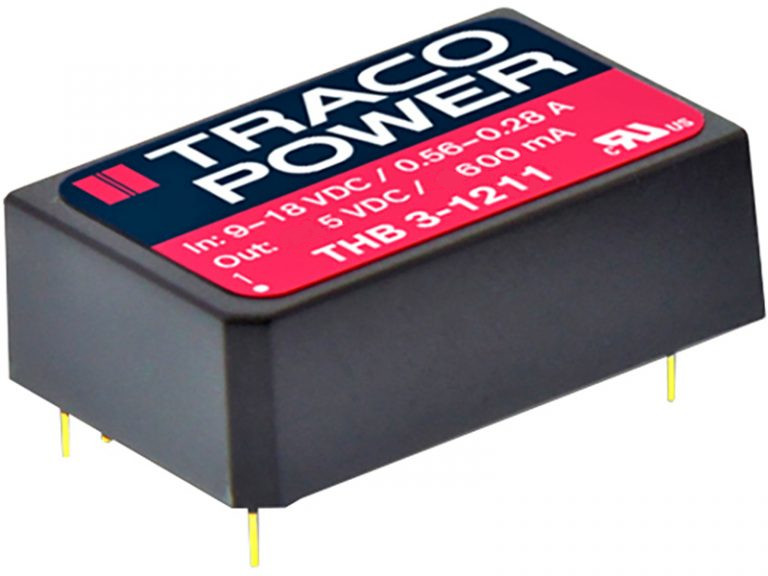
\includegraphics[scale=0.7]{Imagenes/THB3.jpg}
    \caption{Fuente CC-CC aislada THB 3-1211 de Traco Power, en su encapsulado de montaje THT con patas en configuración DIP-24.}
    \label{encapsulado_TRACO}
\end{figure}

La fuente viene en un encapsulado de montaje through-hole, con una configuración de pines compatible con un encapsulado de tipo DIP-24, como se ve en la figura \ref{encapsulado_TRACO}. El dispositivo cuenta con protecciones para conservar su integridad y proteger el resto de los circuitos, como protección contra cortocircuitos y función de undervoltage lockout, que detiene el funcionamiento de la fuente ante la detección de baja tenisón de salida.\\

Para una buena inmunidad al ruido, se conectan externamente a la fuente una serie de capacitores de bypass que se encargan de filtrar los ruidos de altas frecuencias que se introducen por interferencia. Estos incluyen un capacitor de \SI[]{4.7}[]{\micro\farad} en derivación entre la entrada de la fuente y $GND_1$, y luego un paralelo de dos capacitores entre la salida aislada de \SI[]{5}[]{\volt} y $GND_D$, de \SI[]{0.1}[]{\micro\farad} y \SI[]{10}[]{\micro\farad}, para filtrar un amplio rango de frecuencias de interferencia.\\

\subsubsection{Alimentación Digital}

En la mitad inferior de la tabla \ref{tabla:resumen_alimentacion} se encuentran todos los requerimientos de alimentación de la parte digital, que se dividen en dos niveles de tensión:\\

\begin{itemize}
    \item {\SemiBold Circuito de 5 V:} Alimentación del sensor de efecto Hall que consume \SI[]{6}[]{\milli\ampere}, del controlador TMS320F28335 con consumo de \SI[]{300}[]{\milli\ampere}, y del ciruito FTDI para USB FT232BL que requiere \SI[]{25}[]{\milli\ampere}. Consumo total de \SI[]{331}[]{\milli\ampere}. 
    \item {\SemiBold Circuito de 3.3 V:} Únicamente necesario para la alimentación del lado digital del aislador para I\textsuperscript{2}C (ISO7242C), que consume un máximo de \SI[]{24}[]{\milli\ampere}.\\
\end{itemize}

\lipsum[1]\\

\paragraph{Circuito de 5 V}

\lipsum[2]\\

\paragraph{Circuito de 3.3 V}

\lipsum[3]\\